\scanpage{74}
\mspage{73}

\handwritten{7.} Nous verrons çi-dessus que la réponse à la question précédente est affirmative lorsque $k$ est un corps fini, en particulier si c'est le \unsure{coops|corps} premier $\underline{F}_p$, On trouve alors, grâce à cette structure d'extension sur $\underline{G}(\underline{F}_p)$, un homomorphisme canonique de Gerbes (pour tout $k$)
\[
\underline{G}(k)\handwritten{\simeq}\underline{G}(\underline{F}_p)\mathrm{x}_{\deleted{\unsure{\underline{G}(}}\handwritten{\unsure{\underline{\pi}|\underline{\Pi}}}_p(\underline{F}_p))}\handwritten{\underline{\pi}}_p(k)\ ,
\]
et pour $k$ parfait, une réponse affirmative à la question précédente revient à l'assertion que l'homomorphisme précédent est une équivalence de Gerbes. Comme on connait parfaitement bien la Gerbe $\underline{G}(\underline{F}_p)$ et son homomorphisme dans $\handwritten{\underline{\pi}}_p(\underline{F}_p)$ (cf plus bas) cela donnerait donc la structure de $\underline{G}(k)$ en termes de la connai\unsure{a|s}sance de \deleted{$\unsure{\pi|\Pi}_p(\underline{F}_p$} $\handwritten{\underline{\unsure{\Pi|\pi}}}_{\deleted{\unsure{a}}p}(k)$ (connu quand\handwritten{\begin{tikzpicture}[baseline=0cm,x=1cm,y=1cm]\draw[thin] (0,-.45)--(.17,.45);\end{tikzpicture}}on connait $\handwritten{\pi}_1(k)=\operatorname{Gal}(\handwritten{\bar{k}}/k)$) et \deleted{de} l'homomorphisme $\handwritten{\underline{\pi}}_p(k\deleted{\unsure{Fr|F_p}})\handwritten{\longrightarrow\underline{\pi}}_p(\underline{F}_p)$ (connu quand on connait $\handwritten{\pi}_1(k)\handwritten{\longrightarrow\pi}_1(\underline{\unsure{\mathbb{F}|\rlap{$K$}F}}_p)\handwritten{\longrightarrow}\handwritten{\hat{\underline{Z}}}$). Cela résoudrait donc la question de la structure de $\underline{G}(k)$ pour $k$ parfait. On notera que l'objet de Tate de $\mathrm{Fc}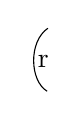
\begin{tikzpicture}[baseline=(r.base),x=1cm,y=1cm]\node[inner sep=0pt] (r) {$\mathrm r$};\draw[thin] (.06,.42)..controls (-.19,.25) and (-.17,-.25)..(.05,-.38);\end{tikzpicture}\mathrm{iso}(k)$ provient de celui de $\mathrm{Fcriso}(\underline{F}_p)$ et sera donc également déterminé. Le foncteur fibre canonique sur $K$\inserted{$=K(k)$}\handwritten{\begin{tikzpicture}[baseline=0cm,x=1cm,y=1cm]\draw[thin] (0,-.3)--(.05,.05)..controls (.1,.16) and (.2,.12)..(.3,.12)--(1.1,.14);\end{tikzpicture}} correspond alors à un foncteur fibre de $\mathrm{Fcriso}(\underline{F}_p)$ sur $K$, un foncteur fibre de \deleted{$\underline{\unsure{\pi|\Pi}}_p(k)$}\inserted{la catégori\unsure{\.{e}|e} des $\underline{Q}_p$-faisceaux constr. sur $k$}\handwritten{\begin{tikzpicture}[baseline=0cm,x=1cm,y=1cm]\draw[thin] (0,-.3)..controls (.08,.18) and (.2,.13)..(.7,.14)--(4,.15)..controls (5.2,.2) and (5.8,-.15)..(7.1,.14)..controls (7.4,.2) and (7.5,.25)..(7.55,.38)--(7.35,.4);\end{tikzpicture}} sur $K$, et un isomorphisme entre les ``restrictions'' de ces foncteurs à la catégorie des $\underline{Q}_p$-faisceaux constructibles sur $\underline{F}_p$ ; or le premier foncteur fibre n'\unsure{\.{e}|e}\unsure{s.|s}t autre que \inserted{celui déduit par}\handwritten{\begin{tikzpicture}[baseline=0cm,x=1cm,y=1cm]\draw[thin] (0,-.4)--(.02,.03)..controls (.08,.2) and (.2,.16)..(.4,.16)--(3.7,.22)..controls (4.1,.12) and (4.15,.5)..(4,.52);\end{tikzpicture}} l'\unsure{\.{e}|e}xtension des scalaires $\underline{Q}_p=K\handwritten{\unsure{\rlap{$-$}(|(}}\underline{F}_p)\handwritten{\longrightarrow}K=K(k)$ du foncteur fibre analogue sur $\unsure{\mathbb{F}|\rlap{$\mathrm{G}$}\mathrm{F}|\mathrm{F}|\mathrm{G}}\mathrm{criso}(\underline{F}_p)$, le deuxième est \unsure{\rlap{h}l|l|h}e foncteur \inserted{\handwritten{$i$:}}\handwritten{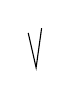
\begin{tikzpicture}[baseline=0cm,x=1cm,y=1cm]\draw[thin] (0,.32)--(.1,-.12)--(.17,.38);\end{tikzpicture}} $V\handwritten{\mapsto}V\otimes_{\underline{Q}_p}K$, et l'isomorphisme \deleted{canonique} entre les restrictions est l'isomorphisme canonique évident\inserted{\handwritten{(compatibilité de $i$ aux changements de corps de base)}}\handwritten{\begin{tikzpicture}[baseline=0cm,x=1cm,y=1cm]\draw[thin] (0,-.3)--(.04,.08)..controls (.3,.14) and (.45,.12)..(.6,.1)--(6.9,.12)..controls (7.1,.1) and (7.18,.18)..(7.2,.35);\end{tikzpicture}}. Donc la structure supplémentaire de $\underline{G}(k)$ (savoir sa section \deleted{sur} canonique sur $K$) est déterminée par la connaissance de la section de $\handwritten{\underline{\pi}}_p(k)$ sur $K$ (i.e. le foncteur précédent $V\handwritten{\mapsto}V\otimes_{\underline{Q}_p}K$ ) et l'isomorphisme de l'\unsure{iamge|image} de ladite section dans $\handwritten{\underline{\pi}}_p(\underline{F}_p)$ avec la section provenant de\deleted{\unsure{s}} la section canonique de $\handwritten{\underline{\pi}}_p(\underline{F}_p)$ sur $\underline{Q}_p$ ; ce sont là des données qui ne sont évidemment pas contenues dans celle du groupe

\margin{\handwritten{\uline{NB} On a donc, en comparant le foncteur ``fibre ``\deleted{\unsure{oubli}} en $\bar{k}$'' sur $Q_p$, et le foncteur précédent, un torseur canonique sur $K$ de groupe \deleted{\unsure{de}}\begin{tikzpicture}[baseline=0cm,x=1cm,y=1cm]\draw[gray,thin] (.12,.47)..controls (-.35,.31) and (-.26,-.35)..(.29,-.36);\end{tikzpicture}lien $\underline{\pi}_p(k)_K$\deleted{\illegible{2} $\unsure{Q_p|\mathbb{Q}_p}$}}}
